\documentclass[12pt,tikz,border=5pt]{article}
\usepackage[margin=1in]{geometry}
\usepackage[spanish]{babel}
\addto\captionsspanish{\renewcommand{\tablename}{Tabla}}
\decimalpoint
\usepackage{tikz}
\usepackage{subcaption}
\usetikzlibrary{babel} 
\usepackage{setspace}
\usepackage{booktabs}
\usepackage{natbib}   
\usepackage{hyperref}
\usepackage{enumitem}
\usepackage{multicol}
\usepackage{amsmath}
\usepackage{amssymb} 
\usepackage{amsfonts}
\usepackage{amsthm}
\newtheorem{ejercicio}{Ejercicio}[section]

\doublespacing

\title{Cálculo Diferencial e Integral \\ Licenciatura en Ingeniería en Computación}
\author{Dr. Julian Bravo \\ M. en C. Edwin Pérez}
\date{\today}

\begin{document}

\maketitle

\section{Modelos Matemáticos}

Ejercicios tomados del libro de Cálculo de una Variable Trascendentes Tempranas 4ta Edición\citep{stewart2001calculo}.

\begin{ejercicio}
  Clasifique cada una de las funciones como función potencia, función raíz, polinomio (indique el grado), función racional, función algebraica, función trigonométrica, función exponencial o función logarítmica.
  \begin{multicols}{3}
    \begin{enumerate}[label=(\alph*)]
      \item $f(x) = \sqrt[5]{x}$
      \item $g(x) = \sqrt{1-x^{2}}$
      \item $h(x) = x^{9} + x^{4}$
      \item $r(x) = \displaystyle\frac{x^{2} + 1}{x^{3} + x}$
      \item $s(x) = \tan{2x}$
      \item $t(x) = \log_{10}x$
      \item $y = \displaystyle\frac{x - 6}{x + 6}$
      \item $y = x + \displaystyle\frac{x^{2}}{\sqrt{x - 1}}$
      \item $y = 10^{x}$
      \item $y = x^{10}$
      \item $y = 2t^{6} + t^{4} - \pi$
      \item $y = \cos{\theta} + \sin{\theta}$
    \end{enumerate}
  \end{multicols}
\end{ejercicio}

\newpage
\begin{ejercicio}
  Haga coincidir cada ecuación con su gráfica. Explique su decisión en cada caso (no utilice calculadora ni graficadora).
  \begin{multicols}{3}
    \begin{enumerate}[label=(\alph*)]
      \item $y = x^{2}$
      \item $y = x^{5}$
      \item $y = x^{8}$
    \end{enumerate}
  \end{multicols}
  \begin{figure}[h!]
      \begin{center}
          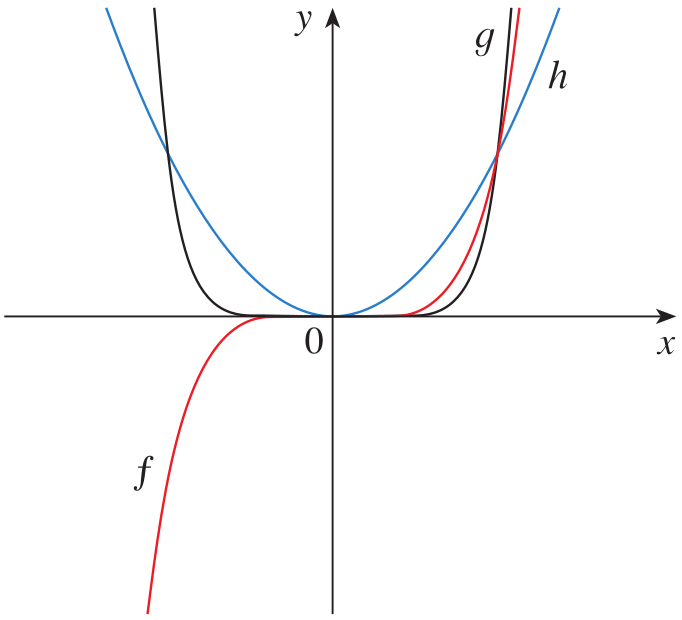
\includegraphics[width=0.30\textwidth]{figures/ejercicio2p2pA.png}
      \end{center}
      \caption{Gráficas de las funciones correspondientes a los incisos $(a)$, $(b)$ y $(c)$.}\label{fig:ejercicio2p2pA}
  \end{figure}
  \begin{multicols}{2}
    \begin{enumerate}[label=(\alph*), start=4]
      \item $y = 3x$
      \item $y = 3^{x}$
      \item $y = x^{3}$
      \item $y = \sqrt[3]{x}$
    \end{enumerate}
  \end{multicols}
  \begin{figure}[h!]
      \begin{center}
          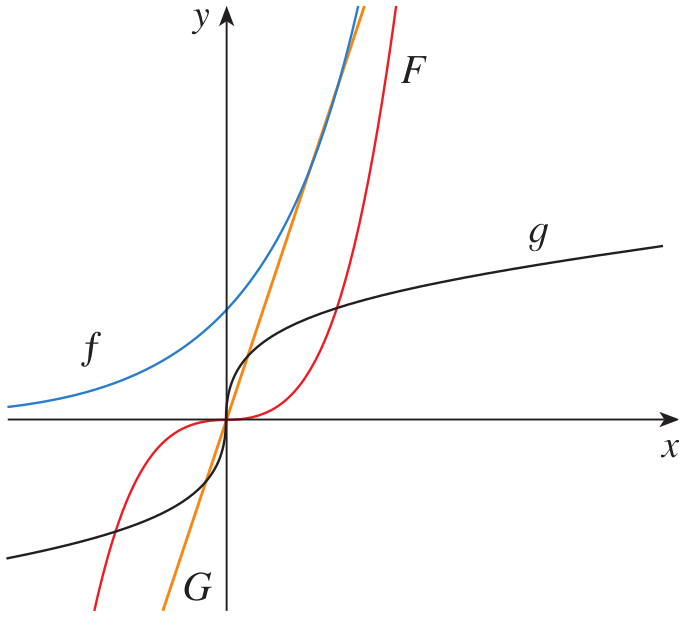
\includegraphics[width=0.30\textwidth]{figures/ejercicio2p2pB.png}
      \end{center}
      \caption{Gráficas de las funciones correspondientes a los incisos $(d)$, $(e)$, $(f)$ y $(g)$.}\label{fig:ejercicio2p2pB}
  \end{figure}
\end{ejercicio}

\newpage
\begin{ejercicio}
  \begin{enumerate}[label=(\alph*)]
    \item Encuentre una ecuación para la familia de funciones lineales con pendiente 2 y trace la gráfica de varios miembros de la familia.
    \item Halle una ecuación para la familia de funciones lieneales tal que $f(2) = 1$ y dibuje varios miembros de la famlia.
    \item ¿Qué función pertenece a ambas familias?
  \end{enumerate}
\end{ejercicio}

\begin{ejercicio}
  El gerente de un bazar de fin de semana sabe con base en experiencias anteriores que si cobra $x$ pesos mexicanos por la renta de espacio en el bazar, entonces el número $y$ de espacios que puede rentar está dado por la ecuación $y = 200 - 4x$.
  \begin{enumerate}[label=(\alph*)]
    \item Trace la gráfica de esta función lineal (recuerde que la renta que se cobra por espacio y el número de espacios que pueden rentarse no pueden ser cantidades negativas).
    \item ¿Qué representan la pendiente, la ordenada al origen y la abscisa al origen?
  \end{enumerate}
\end{ejercicio}

\begin{ejercicio}
  La relación entre las escalas de temperatura Fahrenheit ($F$) y Celsius ($C$) está dada por la función lineal $F = \frac{9}{5} C + 32$.
  \begin{enumerate}[label=(\alph*)]
    \item Trace la gráfica de esta función.
    \item ¿Cuál es la pendiente de la gráfica y qué representa? ¿Cuál es la intersección de $F$ y qué representa? 
  \end{enumerate}
\end{ejercicio}

\begin{ejercicio}
  Los biólogos han notado que la cantidad de chirridos que emiten los grillos de cierta especie está relacionada con la temperatura y la correspondencia parece ser casi lineal. Un grillo produce 113 chirridos por minuto a $70 \, ^{\circ}F$ y 173 chirridos por minuto a $80 \, ^{\circ}F$.
  \begin{enumerate}[label=(\alph*)]
    \item Encuentre una ecuación lineal que modele la temperatura en celsius como una función del número de chirridos por minuto $N$.
    \item ¿Cuál es la pendiente de la gráfica? ¿Qué representa? 
    \item Si los grillos están chirriando a 150 chirridos por minuto, estime la temperatura.
  \end{enumerate}
\end{ejercicio}

\begin{ejercicio}
  Determine, para cada una de las gráficas de dispersión, qué tipo de función elegiría como modelo para la información. Explique sus elecciones.
  \begin{figure}[h!]
    \begin{center}
      \begin{subfigure}{0.2\textwidth}
          \centering
          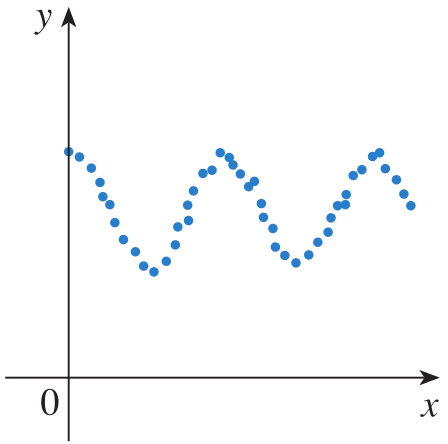
\includegraphics[width=\linewidth]{figures/ejercicio2p7pA.png}
          \caption{}
          \label{fig:sub1}
      \end{subfigure}
      \hfill
      \begin{subfigure}{0.2\textwidth}
          \centering
          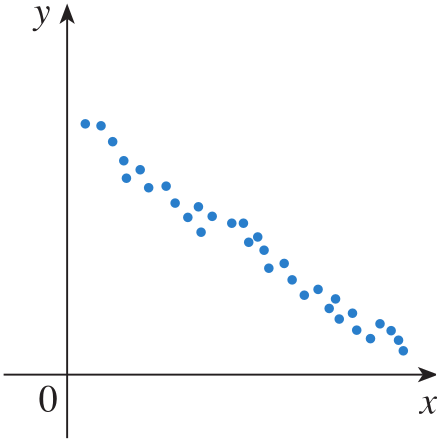
\includegraphics[width=\linewidth]{figures/ejercicio2p7pB.png}
          \caption{}
          \label{fig:sub2}
      \end{subfigure}
      \hfill
      \begin{subfigure}{0.2\textwidth}
          \centering
          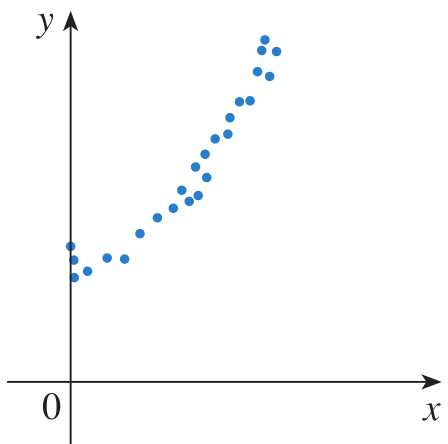
\includegraphics[width=\linewidth]{figures/ejercicio2p7pC.png}
          \caption{}
          \label{fig:sub3}
      \end{subfigure}
      \hfill
      \begin{subfigure}{0.2\textwidth}
          \centering
          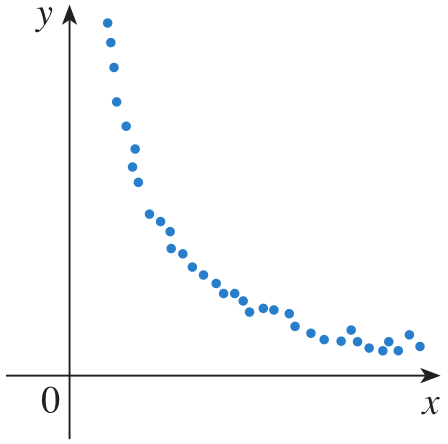
\includegraphics[width=\linewidth]{figures/ejercicio2p7pD.png}
          \caption{}
          \label{fig:sub4}
      \end{subfigure}
    \end{center}
    \caption{Gráficas de dispersión del ejercicio \ref{ejercicioDispersion}.}\label{fig:ejercicio2p7}
  \end{figure}
  \label{ejercicioDispersion}
\end{ejercicio}

\begin{ejercicio}
  Los biólogos han observado que la cantidad de chirridos que emiten los grillos de cierta especie parece estar relacionada con la temperatura. La tabla \ref{tabla:tempChiPerMin} muestra la cantidad de chirridos para varias temperaturas.
  
\begin{table}[!h]
    \centering
    \begin{tabular}{cc}
        \toprule
        \textbf{Temperatura ($^\circ$C)} & \textbf{Chirridos por minuto} \\
        \midrule
       10.00 & 20 \\
       12.78 & 46 \\
       15.56 & 79 \\
       18.33 & 91 \\
       21.11 & 113 \\
       23.89 & 140 \\
       26.67 & 173 \\
       29.44 & 198 \\
       32.22 & 211 \\
        \bottomrule
    \end{tabular}
    \caption{Temperatura y chirridos por minuto}
    \label{tabla:tempChiPerMin}
\end{table}

\begin{enumerate}[label=(\alph*)]
  \item Realice una gráfica de dispersión de la información.
  \item Encuentre y dibuje la línea de regresión.
  \item Use el modelo lineal de la parte (b) para estimar la cantidad de chirridos a $100 ^{\circ}F$.
\end{enumerate}
\end{ejercicio}

\newpage
\begin{ejercicio}
  La tabla \ref{tabla:saltoGarrocha} proporciona las alturas ganadoras en las competencias de salto con garrocha de los Juegos Olímpicos durante el siglo XX.
  
\begin{table}[!hb]
    \centering
    \begin{tabular}{cccc}
        \toprule
        \textbf{Año} & \textbf{Altura (metros)} & \textbf{Año} & \textbf{Altura (metros)} \\
        \midrule
        1900 & 3.30 & 1956 & 4.55 \\
        1904 & 3.49 & 1960 & 4.70 \\
        1908 & 3.70 & 1964 & 5.09 \\
        1912 & 3.95 & 1968 & 5.39 \\
        1920 & 4.09 & 1972 & 5.49 \\
        1924 & 3.95 & 1976 & 5.49 \\
        1928 & 4.19 & 1980 & 5.77 \\
        1932 & 4.31 & 1984 & 5.74 \\
        1936 & 4.34 & 1988 & 6.02 \\
        1948 & 4.29 & 1992 & 5.79 \\
        1952 & 4.54 & 1996 & 5.91 \\
        \bottomrule
    \end{tabular}
    \caption{Altura a lo largo de los años}
    \label{tabla:saltoGarrocha}
\end{table}

\begin{enumerate}[label=(\alph*)]
  \item Dibuje una gráfica de dispersión y determine si un modelo lineal es adecuado.
  \item Encuentre y dibuje la línea de regresión.
  \item Utilice el modelo lineal para predecir la altura del salto con garrocha ganador en los Juegos Olímpicos del año 2000 y compárelo con la altura ganadora real de $5.9\,m$.
  \item ¿Es razonable usar el modelo para predecir las alturas vencedoras en los Juegos Olímpicos del año 2100?
\end{enumerate}
\end{ejercicio}

\bibliographystyle{abbrv}
\bibliography{cite}

\end{document}
